\section{Análise de Memória Volátil}
    
    \vspace{10.5cm}
    
    \hspace{1cm}
    Tradicionalmente, peritos usam a técnica denominada \textit{live forensics} para coletar dados de um computador ligado na rede elétrica \cite{vecchia2019}. No entanto, no contexto corporativo de Resposta a Incidentes, técnicos podem estar interessados em saber que processos estão usando a memória principal, ou apenas duplicar os dados presentes nela naquele momento.
    
    \vspace{4mm}
    
    \hspace{1cm}
    Existem casos em que programas maliciosos dependem apenas da memória principal para funcionar, os chamados \textit{file-less malwares} \cite{wael2018}. Por conseguinte, esse aparato do sistema pode conter informações sobre programas maliciosos que estejam em operação, mas sem fornecer informações suficientes para dizer como esse programa surgiu \cite{luttgens2014}.

    \subsection{Técnicas}
    
    \hspace{1cm}
    Realizar coleta de dados da memória volátil não é uma tarefa tão simples. Deve-se ter em mente qual problema está sendo tratado e quais equipagens compõem o corpo de investigação. Em concordância com \citeonline{ligh2014}, adotaremos o diagrama apresentado pela figura \ref{diagrama_volatile}, para decidir como coletar os dados desejados.
    
    \begin{figure}[H]
    	\centering
    	\caption{Diagrama de decisões para coletar dados em memória volátil}
    	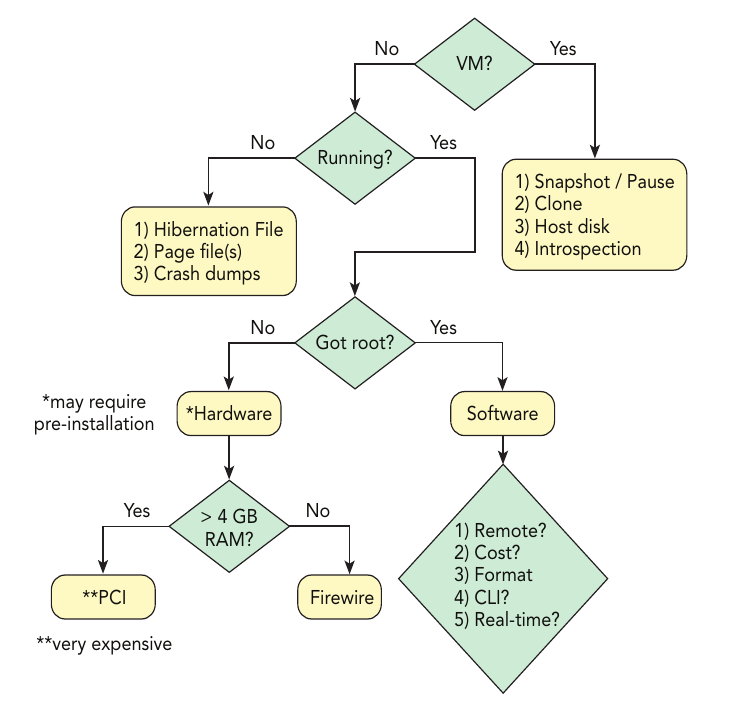
\includegraphics[scale=0.7]{img_volatile_diag}
    	\caption*{Fonte: \citeonline{ligh2014}.}
    	\label{diagrama_volatile}
    \end{figure}
    
    \hspace{1cm}
    Não detalharemos todos os casos que o diagrama busca atender. Focaremos nas decisões tomadas por um perito que queira coletar a memória de um computador, sem ativar mecanismos antiforenses adotados por \textit{rootkits} que possam estar no aparelho \cite{ligh2014}.
    
    \vspace{4mm}
    
    \hspace{1cm}
    Apesar de dispositivos PCI serem caros, como defendem \citeonline{ligh2014}, eles garantem certa segurança na coleta de cópias de memória volátil, por estarem no nível lógico de dispositivos de acesso direto à memória (do inglês DMA ou \textit{Direct Memory Access}). A título de curiosidade, \citeonline{stuttgen2013} mostraram que essa forma de coleta garante que programas maliciosos não consigam adulterar o comportamento de ferramentas como a \textit{FTK Imager}. Ferramentas similares realizam um \textit{snapshot} da memória principal, e armazenam isso em alguma mídia. Dessa forma, se elas forem comprometidas, o perito não consegue prosseguir com o exame pericial.
    
    \vspace{4mm}
    
    \hspace{1cm}
    Para examinar os elementos coletados, devemos identificar qual sistema operacional estava em funcionamento, pois, cada sistema implementa estruturas de dados diferentes para manutenção de suas aplicações. Exemplo disso: o sistema operacional Windows tem um formato de arquivos executáveis chamado PE (\textit{portable executable}). Enquanto isso, executáveis do Linux são mantidos no formato ELF.
   
    \subsection{Ferramentas}

    \hspace{1cm}
    Para examinar artefatos digitais, podemos usar a ferramenta de código aberto Volatility. Ela suporta amostras de memória volátil de sistemas operacionais como Windows, Linux, Mac OS e Android (32 bits) \cite{ligh2014}. Além disso, esta ferramenta permite que pesquisadores criem \textit{plugins} que auxiliem no exame de recursos do sistema até então não suportados, como fizeram \citeonline{case2015}, ao criar diversos \textit{plugins} para exame especializado de diferentes estruturas internas do sistema operacional Mac OS.

    \subsection{Exercícios}
    
    \begin{example}[\quad \large Análise de Memória Volátil] \label{cap3_exercicios}
        \begin{enumerate}
            \item Explique os principais motivos pelos quais peritos podem querer coletar dados em memória volátil.
            \item A análise da memória principal de um computador pode acelerar a resolução de um incidente ? 
            \item Quais ferramentas um perito pode usar para coletar e examinar artefatos digitais ?
            \item Explique como peritos podem coletar uma amostra da memória volátil de um computador infectado por um \textit{rootkit}.
        \end{enumerate}
    \end{example}

\newpage